% Part "data": instance selection and instance noise (Nicodeme's lever).
% Numbers: enquete/results/juliet/nico_data_test.csv (data runs), juliet2_test.csv (BCE+EMA +- noise, Juliet),
% results/comparison_local.csv (BCE and RpGAN + R1 + EMA +- noise, Mac), enquete/data.md (mechanics, collapse counts, DeVries).
% Paired rerun 9/11 (noise_03_e100 vs data_ref_e100, seeds 0-7, 60k updates): enquete/results/juliet/noise_rerun_test.csv.
% Figure: figscripts/data.py -> figures/data_selection_pr.pdf.
\section{Data: instance selection and instance noise}
\label{sec:data}

\textbf{Setup.} Data protocol (Table~\ref{tab:intro-protocol}), raw $G$. Compare FIDs only within a block of Table~\ref{tab:data-results}.

\begin{table}[t]
\centering\footnotesize
\setlength{\tabcolsep}{4pt}
\caption{\textbf{Data lever.} FID$_\text{Inc}$ (mean $\pm$ sd) and P/R (VGG), healthy runs.}
\label{tab:data-results}
\begin{tabular}{@{}lrrrr@{}}
\toprule
Variant & Coll. & FID$_\text{Inc}$ & P & R \\
\midrule
\multicolumn{5}{@{}l}{\emph{Data runs: BCE, no EMA, 120k updates (cluster)}} \\
Reference          & 3/8\rlap{$^a$} & 35.4\,$\pm$\,0.9 & 0.51 & 0.52 \\
Selection 95\%     & 2/5 & 38.2\,$\pm$\,2.7 & 0.49 & 0.48 \\
Selection 90\%     & 2/5 & 35.8\,$\pm$\,3.3 & 0.53 & 0.49 \\
Selection 75\%     & 0/3 & 40.8\,$\pm$\,3.9 & 0.54 & 0.40 \\
Selection 50\%     & 4/8 & 47.8\,$\pm$\,2.9 & 0.56 & 0.32 \\
Noise $\sigma_0{=}0.1$ & 4/8 & 35.5\,$\pm$\,2.5 & 0.52 & 0.52 \\
Noise $\sigma_0{=}0.3$ & 0/3 & 37.0\,$\pm$\,1.6 & 0.51 & 0.52 \\
\midrule
\multicolumn{5}{@{}l}{\emph{Paired rerun: same, 60k updates, seeds 0--7 (cluster)}} \\
Reference          & 3/8 & 55.3\,$\pm$\,2.6 & 0.29 & 0.42 \\
Noise $\sigma_0{=}0.3$ & 1/8 & 54.3\,$\pm$\,3.9 & 0.29 & 0.40 \\
\midrule
\multicolumn{5}{@{}l}{\emph{Common protocol (50k split, 200 epochs), $G_{\mathrm{EMA}}$}} \\
BCE + EMA (cluster)        & 0/3\rlap{$^b$} & 30.0\,$\pm$\,0.2 & 0.56 & 0.54 \\
\quad + noise 0.3         & 2/5 & 30.1\,$\pm$\,1.3 & 0.56 & 0.54 \\
RpGAN + R1 + EMA (Mac)    & 0/3 & 22.1\,$\pm$\,1.3 & 0.59 & 0.59 \\
\quad + noise 0.3         & 0/3 & 21.4\,$\pm$\,0.6 & 0.60 & 0.61 \\
\bottomrule
\end{tabular}
\tabnote{Coll.: collapsed runs (R $<0.01$) / seeds. $^a$0/3 on seeds 0--2 (those of noise 0.3). $^b$0/6 with 3 Mac runs. Mac vs cluster: ${\approx}\,2$ FID.}
\end{table}

\subsection{Instance selection}
\textbf{Method.} Score each training image $x$ of digit $c$ by $s(x) = -(f(x)-\mu_c)^\top \Sigma_c^{-1} (f(x)-\mu_c)$; $f$: 128-d feature of the FID$_\text{CNN}$ network (trained on the same 60k images); $\mu_c, \Sigma_c$: its per-digit mean and covariance. Keep the top 95, 90, 75 or 50\% of each digit.

\textbf{Expected.} Keeping the most typical half of ImageNet: FID 21.4 $\to$ 12.6, P $+0.11$, R $-0.03$~\cite{devries2020}, but with a conditional SAGAN (64$\times$64, halved capacity) and FID in the selection's own space.

\textbf{Observed} (Welch vs reference). No rate wins: 90\% ties ($p = 0.83$), 95\% and 75\% are worse within noise ($p = 0.19$, $0.13$), 50\% is clearly worse ($p = 0.002$). At 50\%, R falls in both feature spaces (VGG $-0.20$, $p < 10^{-6}$; CNN $-0.37$; Fig.~\ref{fig:data-selection-pr}): circularity amplifies the loss, it does not create it. P rises significantly only in the selection CNN; in VGG ($p = 0.22$) it partly reflects easier digits (``1'': 28\% $\to$ 35\% of samples).

\begin{figure}[t]
\centering
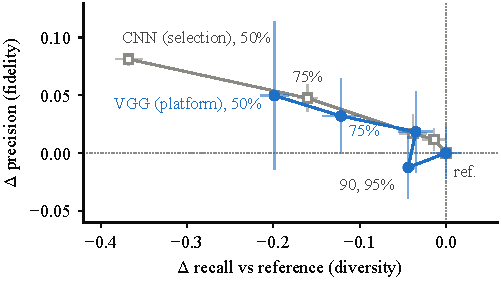
\includegraphics[width=\columnwidth]{data_selection_pr}
\caption{\textbf{Selection costs recall in both feature spaces;} precision gains only in the selection CNN. Change vs the 100\% reference; labels: share kept; bars: sd.}
\label{fig:data-selection-pr}
\end{figure}

\textbf{Why.} (i) The training set stays balanced, yet the unconditional $G$ drops whole digits (``0'': 10.2\% $\to$ 0.0\% at 50\%). (ii) MNIST's tail is likely diversity, not errors: 50\% selection of the \emph{real} images cuts their CNN recall from 0.89 to 0.63. (iii) Capacity is likely not the bottleneck: the same $G$ reaches 22.1 (Sec.~\ref{sec:training}).

\textbf{When it fails.} Already in the paper at 256$\times$256 (BigGAN, 9.8 $\to$ 10.6). Without its random-50\% control (22.8), we cannot separate ``fewer'' from ``chosen'' images.

\subsection{Instance noise}
\textbf{Method.} $D$ sees $x + \sigma_t \varepsilon$, $\varepsilon \sim \mathcal{N}(0, I)$, real and fake (pixels in $[-1,1]$); $\sigma_t$ decays from $\sigma_0$ to 0 at epoch 101 of 200, so FIDs measure only a lasting effect.

\textbf{Expected.} Overlap keeps $D$ imperfect and $G$'s gradient alive~\cite{arjovsky2017,sonderby2017}: stability, no FID gain.

\textbf{Observed.} No significant FID$_\text{Inc}$ effect (Table~\ref{tab:data-results}; Welch $p \ge 0.21$). On raw $G$, noise worsens BCE ($36.6 \to 42.5$, $p = 0.03$; n.s.\ after Bonferroni). No detectable effect on collapses: 2/5 vs 0/6 with EMA (Fisher $p = 0.18$); in the paired 8-seed rerun, 1/8 with noise vs 3/8 without ($p = 0.57$), healthy FID 54.3 vs 55.3 ($p = 0.58$). The earlier ``0 of 8'' with noise does not replicate.

\textbf{Why.} \emph{Collapses are numerical:} all 19 collapsed data runs end with a vanishing gradient for $G$; in 17, $D(G(z)) < 10^{-12}$, where \texttt{BCELoss} clamps its denominator, so the gradient decays as $e^{\text{logit}}$. \emph{Noise does not stop $D$:} one direction separates real from fake, while noise spreads over all pixels~\cite{roth2017}; against the initial $G$, $D$ still reaches 100\% accuracy for $\sigma \le 1$. \emph{With RpGAN}, R1 already is deterministic instance noise~\cite{roth2017,mescheder2018}.

\textbf{When it fails.} Noise ($\sigma_0 \le 0.3$) does not replace a numerically safe loss: \texttt{BCEWithLogitsLoss} keeps the gradient at 1; RpGAN + R1 never collapsed (0/6).

\takeaway{On clean MNIST with an unconditional $G$, data levers do not lower FID$_\text{Inc}$: selection costs recall; noise neither helps nor prevents collapses, which are numerical (sigmoid + \texttt{BCELoss}).}
